%
% Title.tex
% Title Page.
%
% LulzBot® TAZ User Manual
%
% Copyright (C) 2015 Aleph Objects, Inc.
%
% This document is licensed under the Creative Commons Attribution 4.0
% International Public License (CC BY-SA 4.0) by Aleph Objects, Inc.
%

% clear the page style
\date {}
\thispagestyle{empty}
\begingroup
\centering 

%%%% MINI TITLE   %%%%
%\begin{comment}
\begin{center}
%%{\huge \scshape TAZ Six User Manual}
\fontspec{Outage.ttf}\fontsize{24pt}{1em}\selectfont LulzBot Mini User Manual
\end{center}
%\end{comment}

%%%% TAZ TITLE   %%%%
\begin{comment}
\begin{center}
%%{\huge \scshape TAZ Six User Manual}
\fontspec{Outage.ttf}\fontsize{24pt}{1em}\selectfont LulzBot TAZ
%%%\fontspec{Titillium-BoldUpright.otf}\fontsize{24pt}{1em}\selectfont 6

\includegraphics[keepaspectratio=true,angle=0,height=0.03\textheight]{outage-6.png}
\fontspec{Outage.ttf}\fontsize{24pt}{1em}\selectfont User Manual
\end{center}
\end{comment}

\par


%\vspace*{0.1\textheight} 
%%% SET TITLE FONT

%\includegraphics[keepaspectratio=true,angle=0,height=1.0\textheight,width=1.0\textwidth]{TAZ_6_Angle.JPG}

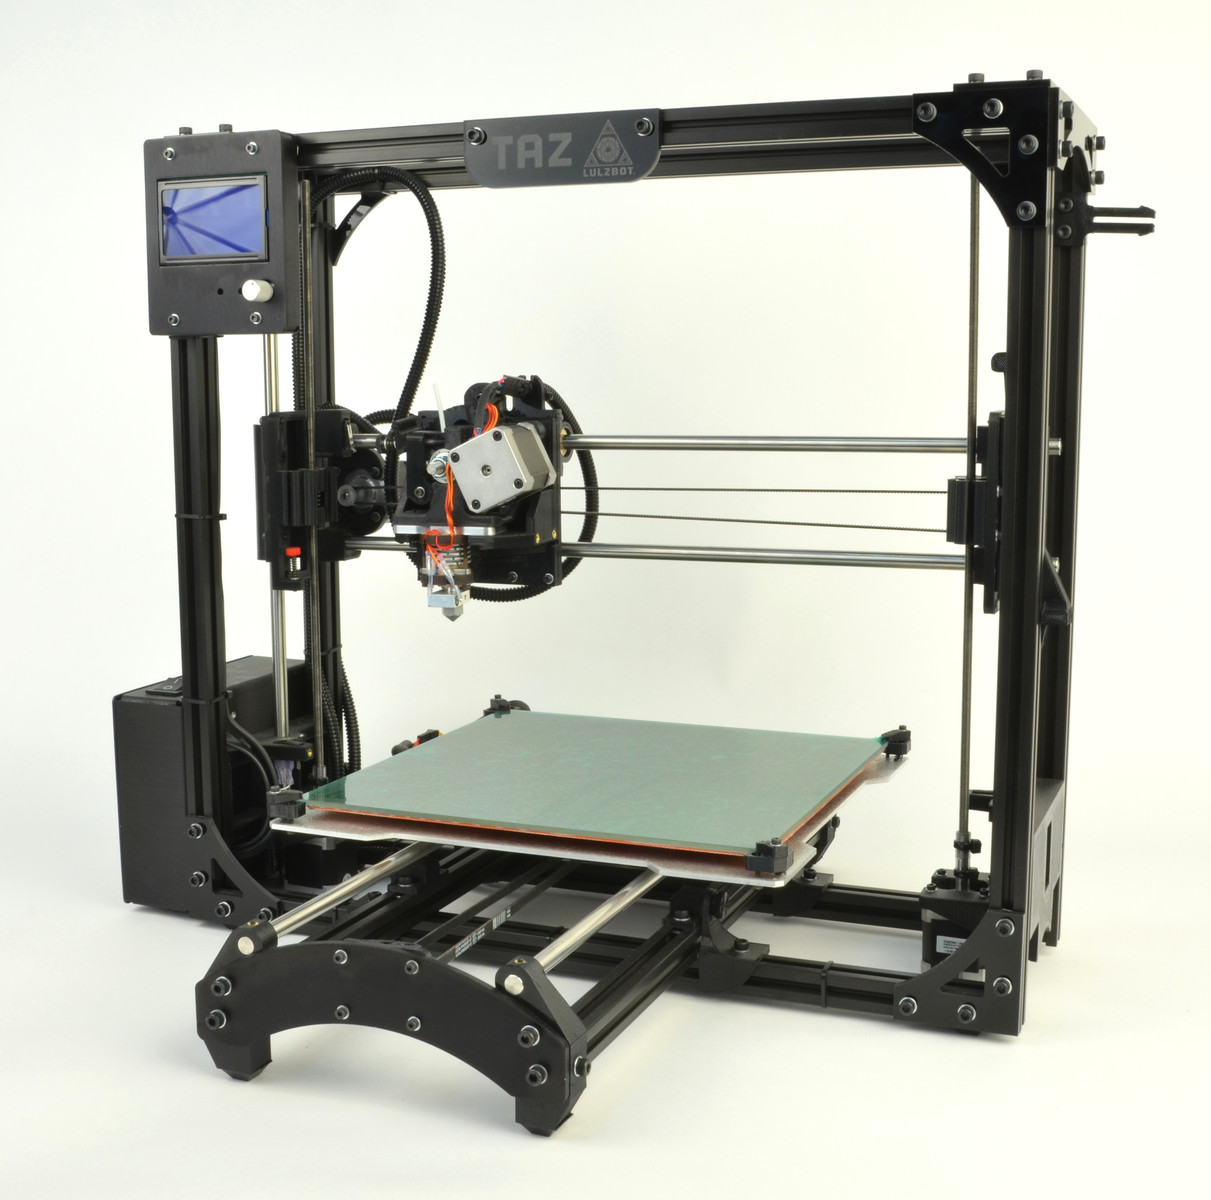
\includegraphics[keepaspectratio=true,angle=0,height=1.0\textheight,width=1.0\textwidth]{taz.jpg}


%\null\vfill
%\rule{0.4\textwidth}{0.4pt}
%\par
\begin{center}

\includegraphics[keepaspectratio=true,angle=0,height=0.25\textheight,width=0.25\textwidth]{Lulzbot_Logo_R_CMYK.eps}

{\large \itshape Aleph Objects, Inc.}
\end{center}
\endgroup
%\vspace*{0.1\textheight} 
%\newpage
%\clearpage
